\section{Results}\label{sec:results}

\subsection{Completed engineering checks and their scope}\label{sec:engineering}
The completed preparation uses a projection of the public HIGGS data, four tool families, three contribution-size strata and 20 logical partitions. A declared deterministic controller performs three weighted federated updates for training requests, feeding each aggregate update into the next step. This is a derived workflow extension of the one-step source question bank, not evidence of autonomous multi-round agent planning. The final-test partition has not been executed.

The current implementation passes 257 software regression tests, with one optional-Torch skip. A TRAIN calibration covered 15 configurations, 12 family--size strata and two repetitions (360 trials); 349 trials passed the reference and transport-validity checks. All five baseline configurations passed their 24 trials. The zero-bias DP and combined configurations failed five and six trials, respectively; these failures are retained, rather than removed or repeated until successful. A shortlist was frozen from TRAIN before evaluating SELECT. Of 216 SELECT trials, 215 passed: the lower-bias combined candidate failed one fixed-horizon completion check. The functional/cost rule therefore selected DP bias multiplier 1 and combined bias multiplier 2. This selection minimises framed plaintext cost among the eligible candidates; it is not an empirical validation of the attacker- and energy-budget controller in \cref{alg:controller}.

\begin{table}[t]
\centering
\caption{Completed Mac engineering validation. Byte figures are mean TLS plaintext including application framing, not observed IPv4 traffic or measured energy.}\label{tab:engineering}
\footnotesize
\begin{tabular}{@{}lrr@{}}
\toprule
SELECT configuration & Passed/trials & Mean MB/session \\
\midrule
Minimal TLS RPC & 24/24 & 0.006161 \\
Unshaped with all-site controls & 24/24 & 0.337332 \\
Padding & 24/24 & 0.348878 \\
Rounds and cover sites & 24/24 & 0.376140 \\
DP, bias multiplier 1 & 24/24 & 78.184944 \\
Combined, bias multiplier 2 & 24/24 & 136.077084 \\
\bottomrule
\end{tabular}
\end{table}
The DP candidates use the arrival variant with a 10\,s horizon, 0.5\,s ticks, $\varepsilon_{\mathrm{dir}}=0.2$, an input cap of 8192 bytes and $\Delta=16384$ bytes. These functional comparisons do not establish a measured privacy gain. The difference between minimal TLS and the all-site-control baseline also shows why framing and control traffic must be reported explicitly.

Two local models, \nolinkurl{mistral-small3.1:24b} and \nolinkurl{qwen2.5:14b-instruct-q4_K_M}, each passed 12 TRAIN and 12 SELECT typed-plan, tool-result and structured numerical-summary checks in the repaired validation. Before freezing this version, each model failed two TRAIN summaries by dropping the exponent of a small coefficient. The repaired presentation supplies plain decimal JSON numbers; the numerical comparison tolerances were not relaxed, and previous failures remain archived. These 48 passing checks establish consistency for this bounded workflow, not general free-text answer quality, hosted-model robustness or autonomous replanning.

Result preservation was checked by restoring 1292 eligible files and comparing their hashes independently; calibration hashes before and after the model-only work matched. Private TLS keys were excluded from the evidence backup. No physical energy measurement, edge-device comparison, final-test attacker result or 10\,Gbps NetShaper result follows from these checks. The four-role EC2 tunnel represents one physical data endpoint and a multiplexed observer link; it does not instantiate 20 independently observed physical sites.

\subsection{Four-instance network validation}\label{sec:cloudresults}
All 168 sessions in the seven-mode, three-step-workflow campaign passed independent reference checks and transport-validity checks. Every phase committed, all 168 session replicas were acknowledged by T4, and cleanup recorded no error. Captures at both ends covered every session and reported zero kernel drops. These are functional and acquisition-validity results, not a measured privacy guarantee.

\begin{table}[t]
\centering
\caption{Four-instance EC2 validation: 24 successful sessions per mode. IPv4 bytes include headers and ACKs on the T2--T3 segment. Latency includes the public 1\,s start lead. MB denotes $10^6$ bytes.}\label{tab:cloudcost}
\footnotesize
\setlength{\tabcolsep}{3pt}
\begin{tabular}{@{}lrrr@{}}
\toprule
Mode & MB/session & Tool median (s) & Tool p95 (s) \\
\midrule
Unshaped + controls & 0.349353 & 1.123 & 1.372 \\
Padding & 0.360476 & 1.126 & 1.385 \\
Rounds & 0.392321 & 2.011 & 4.011 \\
DP (bias 1) & 78.432703 & 3.070 & 7.953 \\
Combined (bias 2) & 137.468508 & 3.575 & 9.068 \\
NetShaper disabled & 0.395938 & 1.178 & 1.593 \\
NetShaper enabled & 1.313787 & 1.313 & 1.682 \\
\bottomrule
\end{tabular}
\end{table}

\begin{figure*}[t]
\centering
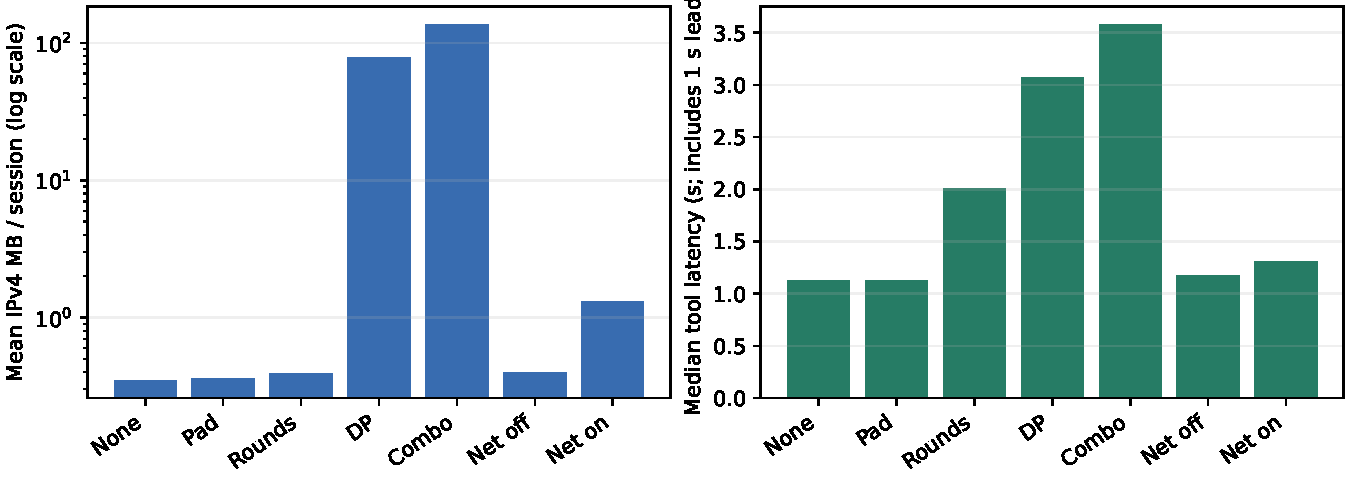
\includegraphics[width=0.94\textwidth]{audit_and_code/outputs/paper_completion_20261022/network_costs.pdf}
\caption{Observed resource costs in the descriptive EC2 campaign. The byte axis is logarithmic. These bars do not compare equal privacy or physical energy, and the seven modes ran in separate phases.}\label{fig:cloudcost}
\end{figure*}

The DP and combined configurations average 78.433 and 137.469\,MB per session on the observed link, respectively, compared with 0.349\,MB for the unshaped all-site-control baseline. Padding averages 0.360\,MB and rounds 0.392\,MB. The large DP cost remains visible after reducing the bias relative to the older pilot: it is a resource trade-off, not evidence that the selected configurations provide a better privacy--energy balance. Median fixed-horizon session completion is approximately 11\,s including the start lead, whereas the tool result can arrive earlier; the tool-latency column must not be used as the session's full protected duration.

NetShaper enabled averages 1.314\,MB within session windows, but continuous cover also exists between sessions and during setup and teardown. At T2, 31.520\,MB is outside the 24 session windows, compared with 31.531\,MB inside; the corresponding outside-window T3 count is 22.348\,MB because the full capture extents differ. We retain and report these bytes rather than equating session-window cost with deployment-wide cost. Without matched privacy accounting, the lower NetShaper byte cost cannot establish a stronger or weaker privacy guarantee.


\subsection{Retrospective cost decomposition and leakage diagnostic}\label{sec:retrospective}
We reanalyse the retained campaign without acquiring further sessions or opening the reserved final-test bank. The all-site-control baseline spends a mean 97.625\% of framed plaintext on control messages, versus 94.558\% for padding and 87.902\% for rounds. These fractions refer to application counters; they do not assign individual encrypted IPv4 packets to plaintext categories. For NetShaper enabled, 49.991\% of T2's full-capture IPv4 bytes fall outside the aligned session windows. Dividing the entire capture by its 24 sessions gives 2.627\,MB per session, compared with the in-window 1.314\,MB. This allocation includes the recorded setup and gaps and is not a steady-state estimate at arbitrary request rates.

Question-cluster bootstrap resampling (4000 draws, averaging each question's two repetitions) gives descriptive 95\% intervals of [1.025, 1.039] for the padding byte ratio, [1.085, 1.162] for rounds, [219.94, 229.08] for DP and [387.59, 398.64] for combined, relative to controls. These intervals are conditional on the acquired questions and phases; they do not remove fixed-order, host-load or temporal confounding.

We also run a fixed random-forest diagnostic using IPv4 byte and packet counts, directional bytes, packet-size statistics, inter-arrival statistics, observed packet span and 22 half-second byte bins. Labels come only from the TRAIN question manifest. Question identifiers, absolute epochs, plaintext payloads, driver tool-completion times and site identities are excluded from features. Family classification uses three leave-one-requested-size-out folds; size classification uses four leave-one-family-out folds. Both repetitions of a question remain on the same side of every split. The forest uses 100 trees, depth four, minimum leaf size two and balanced class weights, with no hyperparameter selection for this retrospective diagnostic. A byte-only forest and a majority classifier are retained as ablations.

\begin{table}[t]
\centering\footnotesize
\caption{Exploratory question-disjoint metadata classification on the multiplexed link. Each mode has only 12 questions (24 sessions). BA is balanced accuracy. Family intervals are conditional 95\% question-cluster bootstrap intervals for fixed out-of-fold predictions, excluding model-refitting uncertainty.}\label{tab:diagnostic}
\begin{tabular}{@{}lrrr@{}}\toprule
Mode & Family BA & Interval & Size BA \\\midrule
Unshaped + controls & 0.500 & [0.250, 0.708] & 0.333 \\
Padding & 0.417 & [0.208, 0.625] & 0.167 \\
Rounds & 0.583 & [0.500, 0.667] & 0.458 \\
DP & 0.292 & [0.167, 0.417] & 0.417 \\
Combined & 0.208 & [0.042, 0.375] & 0.250 \\
NetShaper disabled & 0.292 & [0.125, 0.375] & 0.375 \\
NetShaper enabled & 0.375 & [0.167, 0.583] & 0.250 \\
\midrule
Chance/majority BA & 0.250 & --- & 0.333 \\\bottomrule
\end{tabular}\end{table}

\begin{figure*}[t]\centering
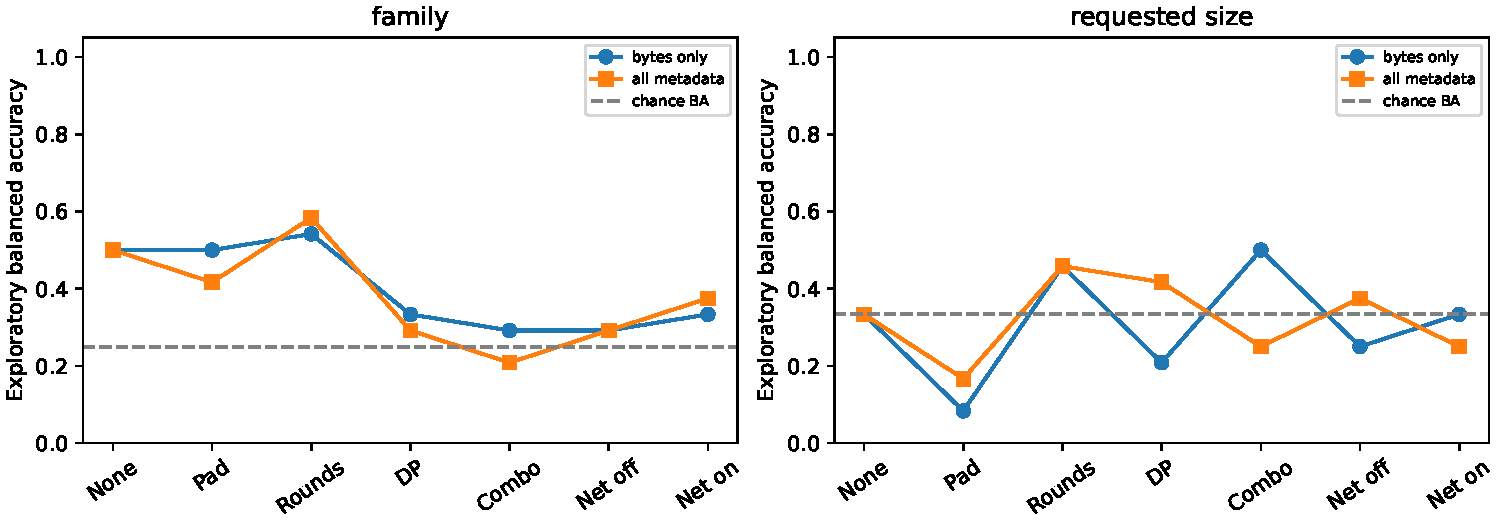
\includegraphics[width=.93\textwidth]{audit_and_code/outputs/evaluation_extension_20261022/attacker_diagnostic.pdf}
\caption{Retrospective byte-only and all-metadata random forests under question-disjoint cross-validation. Session segmentation is supplied by the retained acquisition windows. This is an exploratory diagnostic, not a final-test privacy ranking.}\label{fig:diagnostic}
\end{figure*}

Combined's family BA is 0.208 versus 0.500 for controls, whereas rounds reaches 0.583. This suggests that byte cost alone does not order the tested classifier's performance. It does not establish a privacy improvement: the small bank contains one acquired question per family--size stratum, modes occupy separate phases, and the session windows are oracle supplied rather than inferred by an observer. Requested size denotes the manifest's workload stratum, not a secret per-site contribution label. Near- or below-chance results can reflect insufficient training or distribution shift. No per-site participation result, adaptive attacker search or confirmatory final-test claim follows.

\subsection{Public-contract reliability and resource admission}\label{sec:stress}
The earlier fixed-arrival sweep (2592 cells, 128 draws each) and 90000 independent-seed checks are retained in the artifact. All three pilot-selected bias-eight configurations produced validation overflow, eight cases in total. We therefore evaluate certificates from \cref{prop:contract}, keeping the synthetic results separate from the 168 cloud sessions.

A predeclared grid has 96 synthetic deployments: $N\in\{3,10,20\}$ logical sites, $K\in\{10,20\}$ ticks, $M\in\{1,3\}$ occupied-tick caps, homogeneous or heterogeneous node profiles, total session $\varepsilon\in\{1,4\}$ and completion target $\rho\in\{0.01,0.001\}$. Each direction receives $\varepsilon/(2N)$ and $\Delta=2V$. Heterogeneous volume caps cycle through 1024, 8192 and 32768 bytes. Nonnegative weighted-byte and tick-activity costs are synthetic proxies, not joules. Budgets are constructed stress cases relative to the uniform-contract certificate, with tight and loose nodes and an additional public scaling sweep; admission rates are conditional on this design.

We compare fixed bias eight, zero-observed-failure pilot selection, a conservative $K$-tick certificate, the sharper $M$-tick certificate and per-node risk allocation. Every stochastic policy is ablated with and without a public release cap $C=V$, retaining its bias allocation across that ablation. Periodic constant cover is mandatory: it has an identical abstract frame transcript across private arrivals and is stronger than a positive-$\varepsilon$ bound in this observation model. Candidates are not selected using the new validation draws.

At the base synthetic budgets, uncapped $M$-based uniform admission succeeds in 48/96 scenarios and allocated risk in 56/96, versus 0/96 for the conservative $K$-based rule. The mean ratio of the $M$-based expected-byte upper bound to the $K$-based bound is 0.798. Allocation may increase total cost to relieve a constrained node; it is not a universal reduction in aggregate bytes. Constant cover fits all 96 cases and costs substantially less than uncapped DP in this grid. Capped DP approaches constant-cover cost. Thus the experiment does not support superiority of uncapped Laplace shaping; it identifies the importance of public caps and of a strong cover baseline.

The predeclared validation subset has 252 policy--pattern cases and 1260000 new-seed synthetic deployments with early, spread or last-tick arrivals. Four correlated pointwise 95\% intervals initially have lower limits above the mathematical bound. We retain them and freeze an additional implementation diagnostic of 200000 fresh draws for each flagged case, without changing any parameter. All four new intervals include their exact last-tick probability; the replication adds 800000 draws. These sampling checks do not prove the bound or establish empirical wire privacy. All raw flags, intervals, seeds and certificates remain available.

\begin{figure*}[t]\centering
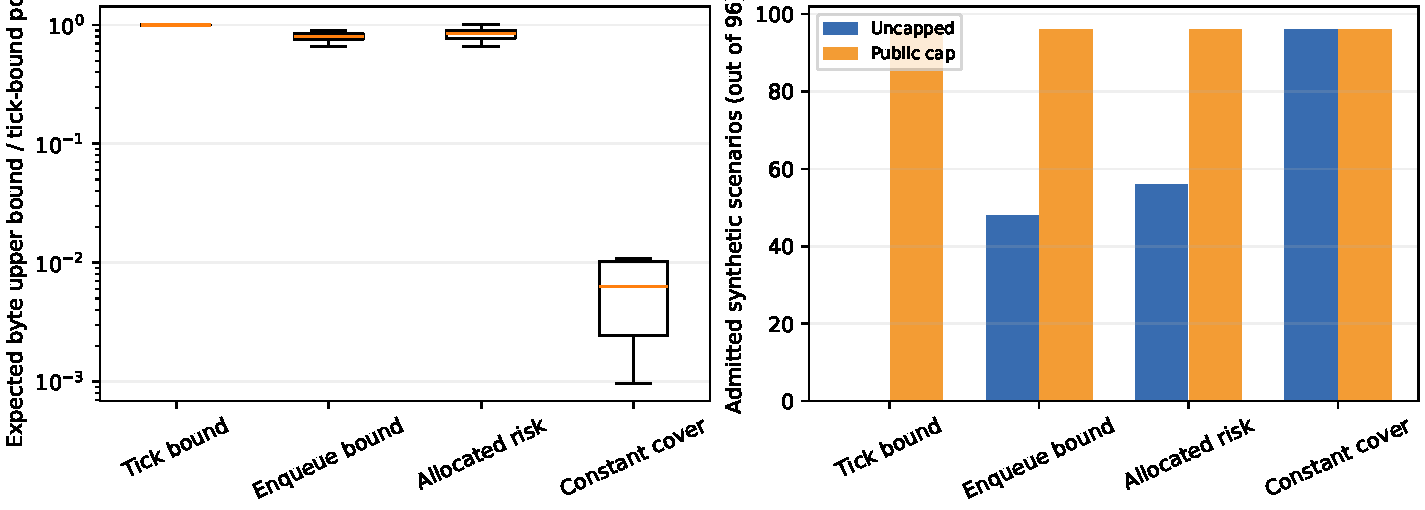
\includegraphics[width=.93\textwidth]{audit_and_code/outputs/reliability_controller_20261023/reliability_admission.pdf}
\caption{Synthetic public-contract admission. Left: distribution of expected-byte upper bounds relative to the conservative tick-count certificate. Right: base-budget admissions with and without public release clipping. Constant cover has a stronger abstract privacy certificate; no physical-energy or equal-cost superiority is inferred.}\label{fig:admission}
\end{figure*}

We separately project a public workflow envelope against periodic constant cover at identical per-direction frame caps. The 32 scenarios vary 3 or 20 logical sites, round cap 3 or 5, interval 0.1 or 0.5\,s, compute bound 0.2 or 1\,s and homogeneous or heterogeneous reply caps. Actual rounds, site participation and delays vary privately within each public envelope. There are 5000 synthetic job instances per scenario (160000 total); 1024 instances are also checked through the scalar contract implementation. A deliberately over-bound job in every scenario is rejected internally without expanding the abstract scheduled transcript. This study uses zero delivery delay; the implementation exposes a public delivery-bound parameter, but network-delay calibration is still required.

The workflow envelope uses 0.077--0.385 times the application bytes of periodic cover, a projected reduction of 61.5--92.3\%, while its projected tool p95 is 1.182--1.786 times the periodic baseline. All these byte counts are fixed by the public schedules, and both baselines have an input-independent abstract transcript. The result is a resource--latency trade-off from fewer public cover slots, not a demonstrated packet-level privacy gain or a measured system speedup. It relies on bounded planning, computation, delivery and frame volume; the current LLM and cloud acquisitions have not established those new contracts.

\begin{figure*}[t]\centering
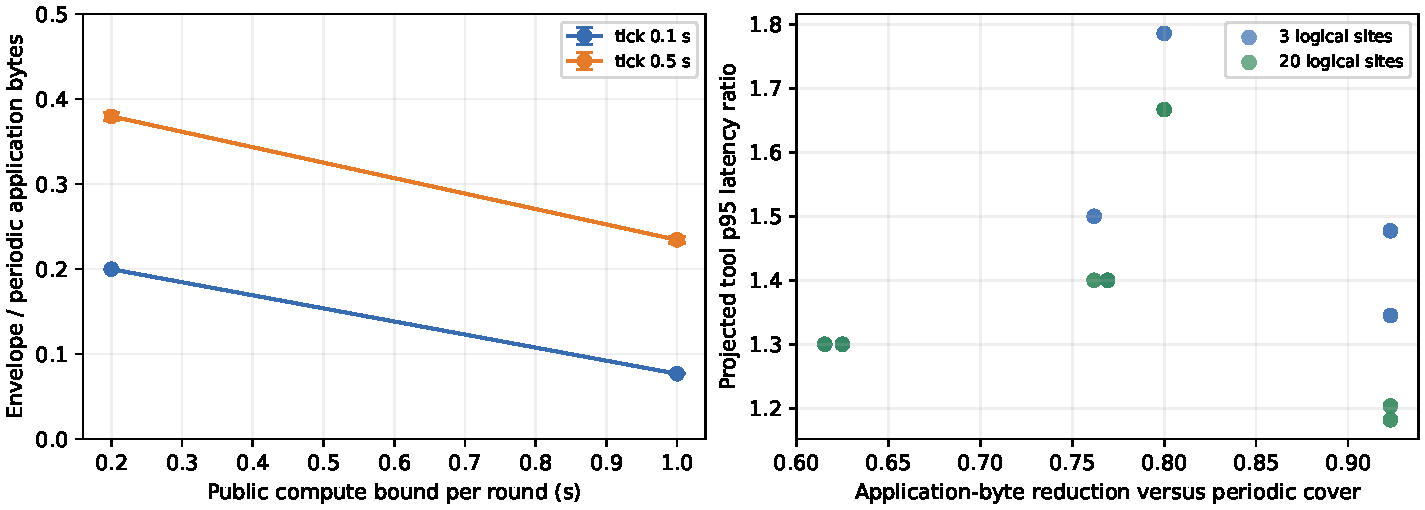
\includegraphics[width=.93\textwidth]{audit_and_code/outputs/reliability_controller_20261023/workflow_envelope_tradeoff.pdf}
\caption{Public-envelope projection against periodic constant cover: byte ratios over compute/tick bounds (left) and projected tool-p95 latency trade-offs (right). Sites are simulated, inputs stay inside declared bounds and delivery delay is zero. These are application-frame models, not EC2 wire measurements.}\label{fig:envelopetradeoff}
\end{figure*}

\subsection{Paired public-contract TLS acquisition}\label{sec:localtls}
The final local frequency comparison runs 32 new SELECT jobs under three policies (96 positive sessions) and ten deliberately invalid jobs under each (30 stress sessions). All 96 complete reference-correct within their frame and timing gates. All 30 violations---over-bound planning or computation, missed reply deadlines, and oversized calls or replies---are reported while fixed cover continues. The capture has 17054 packets, 378 connections, zero reported kernel drops and no unassigned packets; 261 evidence files pass hash checks. These are three logical sites on one physical host under recorded background load.

\begin{table}[t]\centering\small
\caption{Final paired loopback acquisition, 32 fresh scripted jobs per policy. IPv4 costs include the complete TLS lifecycle; tool completion is internal, while every public session retains the full 0.6\,s horizon.}\label{tab:localcontract}
\setlength{\tabcolsep}{5pt}
\begin{tabular}{lrrr}\toprule
Policy & Mean IPv4 (KiB) & Tool p95 (s) & Success \\
\midrule
Workflow envelope & 31.35 & 0.610 & 32/32 \\
Periodic, 6 ticks & 47.05 & 0.610 & 32/32 \\
Periodic, 10 ticks & 68.01 & 0.370 & 32/32 \\
\bottomrule\end{tabular}
\end{table}

Relative to six-tick periodic cover, the envelope's mean captured-byte ratio is 0.6662 (paired 95\% interval 0.6660--0.6664), and its tool-p95 ratio is 1.0004 (0.9986--1.0021). Against ten ticks the byte ratio is 0.461 but tool p95 is 1.649 times as long. Thus frequency choice materially changes the apparent gain: the coarser baseline reduces the saving to 33.4\%, compared with 53.9\% against ten ticks. These narrow intervals omit host and contract-selection uncertainty. Savings relative to these full-frame periodic baselines do not establish optimality over arbitrary public direction schedules or measured energy savings.

The artifact also retains an earlier phase with 63/64 positive sessions and 20/20 correctly reported stress cases: one reference-correct periodic session lost received cover frames and fails acquisition. TLS read/write operations were then serialised without blocking the sending clock on a read; a fresh-seed replication using the unchanged contract passes 64/64 positive and 20/20 stress gates. No failed run is replaced. The final frequency study uses another seed offset and keeps this repair fixed. No wire-privacy certificate, distributed-site result or empirical 0.001 completion-risk claim follows from these sample sizes.

\subsection{Capture agreement and result preservation}
Six modes match packet fingerprints exactly within the aligned session windows at both observation points. Rounds differs by two 52-byte pure ACKs at one session boundary: they are observed 20.5\,$\mu$s before the client end timestamp at T2 and 54.6--56.5\,$\mu$s after it at T3. Both ACKs are present in the full captures, whose fingerprint multisets and total byte counts match. The 104-byte window discrepancy is retained; it is not reported as payload loss or silently corrected. Clock screening and lifecycle coverage reduce acquisition ambiguity but do not eliminate timestamp-boundary sensitivity.

The compact campaign handoff was checksum-verified on the controller. All 14 raw captures were independently copied and SHA256-verified, totalling 226065099 stored pcap bytes; this storage size is distinct from the IPv4 traffic totals in \cref{tab:cloudcost}. Together with the 1292-file restore drill and unchanged calibration hashes, this provides recoverable evidence for the reported engineering results. The evidence does not include physical power measurements or a confirmatory final-test attacker evaluation.
